\chapter{Theory Background}
\section{Introduction}
Cryptanalysis is the technique of extracting useful information about the key by observing the plaintext and cipher text using cryptanalysis try to break the secrecy provided by the cipher. There is no fixed method for cryptanalysis and every cipher is a different challenge to the attacker and hence demands different insight to attack\cite{jha2011cryptanalysis},The study of cipher text in an attempt to restore the message to plaintext is known as cryptanalysis. Cryptanalysis is equally mathematically challenging and complex as cryptography. Because of the complexity involved with cryptanalysis work this document is only focused on the basic techniques needed to decipher monoalphabetic encryption ciphers and cryptograms\cite{smith2001basic}.
In this chapter, explained the history of cryptanalysis, the technology of cryptanalysis, transposition cipher, substitution cipher and description genetics algorithm (GA).

\section{Cryptanalysis}
Cryptanalysis is the technique of deriving the original
message from the ciphertext without any prior knowledge of
secret key or derivation of key from the ciphertext. A general
technique for cryptanalysis, applicable to all cryptographic
algorithms is to try all the possible keys until the correct key
is matched, it is known as exhaustive key search. With every
passing day, the computing ability of hardware is increasing
manifold; therefore it becomes necessary to use long keys for
avoiding exhaustive key search \cite{bokhari2012cryptanalysis} and till today, many cryptanalytic attacks are developed based on these. Each variant of these have different methods to find distinguisher and
based on the distinguisher \cite{khurana2015variants}.

\begin{figure}[h]
	\centering
	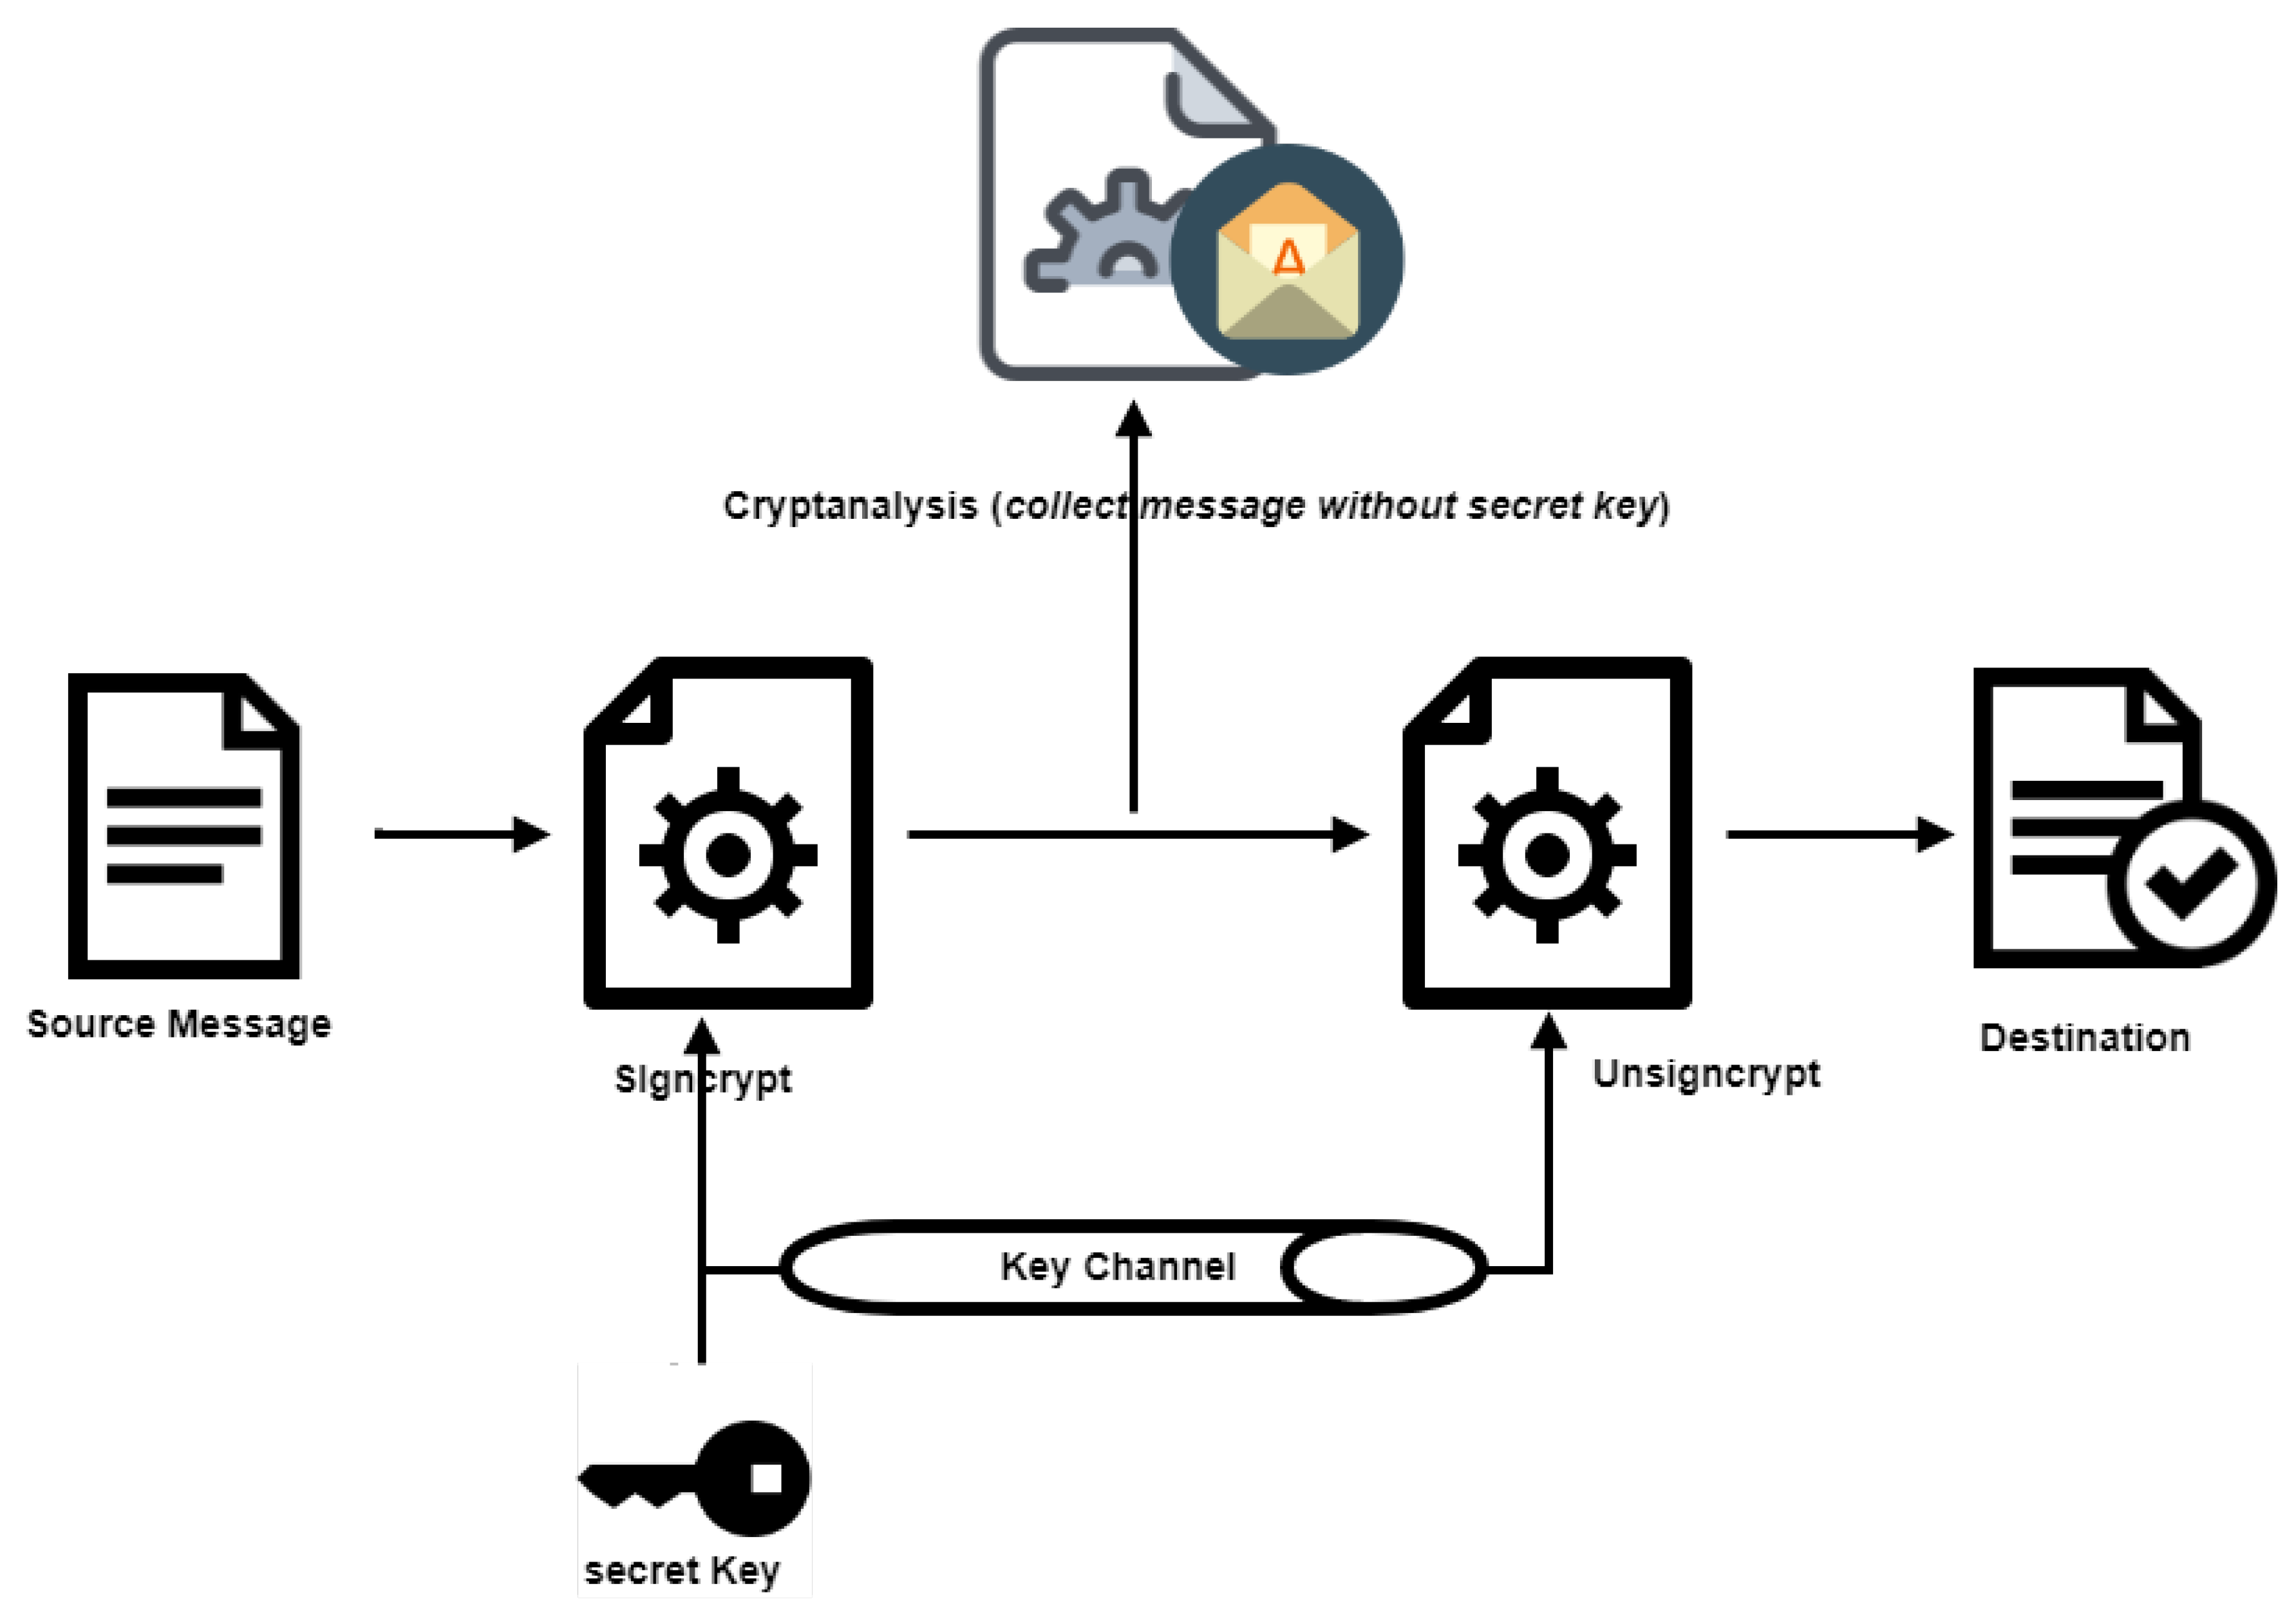
\includegraphics[scale=0.45]{imagenes/cryimage.png}
	\caption{Cryptanalysis cipher text}
\end{figure}

\subsection{CLASSIFICATION OF ATTACKS}

The main goal of a cryptanalyst is to obtain maximum
information about the plaintext (original data).Classification
of attacks can be done on following basis \cite{stallings2006cryptography}:
\begin{enumerate}
    \item{\textbf{Cipher text only attacks:} This is the most powerful attack. The
    attacker has only the knowledge of cipher text. This type of attack is
    successful only on the weakest of the ciphers.}
    \item{\textbf{Known plaintext attack:}attacker has the knowledge of plaintext and the corresponding cipher text, e.g. if an attacker is eavesdropping then  he can also guess the plaintext corresponding to some cipher texts depending upon the position or state of communication, in other words,  In this type a cryptanalyst have plaintext and their corresponding cipher text . Attacker tries to find out the relation between these two.}
    \item{\textbf{Chosen plaintext:}the attacker can choose its plaintext and get the cipher text corresponding to those chosen cipher text or The attacker obtain the various ciphertext corresponding to an arbitrary set of plaintext. }
    \item{\textbf{Chosen cipher text:} attacker is able to get the decrypted plaintext
    corresponding to his choice of cipher text. This attack is same as the
    chosen plaintext, but in a reverse direction which means The attacker obtain the various
    plaintext corresponding to an arbitrary set of cipher text}
    \item{\textbf{Adaptive chosen plaintext:}attacker first observes a large number of cipher texts. Based on the distribution of the cipher texts the attacker chooses a plaintext to get the corresponding cipher text which means the attacker chooses
    subsequent set of plaintext which is based on the information
    obtain from previous encryption methods.}
    \item{\textbf{Related Key: } This is a relatively new attack model. Here the attacker
    can encrypt two plaintext (same plaintext or the two plaintexts with a
    constant difference) with two keys, which have a fixed relation Between each other. This attack model is very weak as there is very little
    chance for the attacker to get encryption with two keys with a Constant
    relation. For lightweight block ciphers as the key is written to the device,
    this type of attack is not very probable.}
\end{enumerate}
\newpage
\subsection{Cryptanalytic technique}
In this section we will explain various cryptanalytic technique. As said earlier that, there are no fixed methods for cryptanalytic techniques for any block ciphers. But there are some methods which can be applied to every ciphers with some variation, though there can not be any guarantee that these methods may break the cipher. Cipher designers apply these methods to analyze security level for the computational security. Informally, broadly classify these techniques as brute force techniques non-brute force techniques. As the name suggest brute force techniques involves search of entire key space. Other techniques utilize the weakness in the structure of the ciphers to find key bits \cite{jha2011cryptanalysis}.

\subsubsection{Brute force technique:}
A brute-force attack is a can be used to attempt to decrypt any
encrypted data. Such an attack might be used when it is not possible to take
advantage of other weaknesses in an encryption system (if any exist) that
would make the task easier. When password guessing, this method is very
fast when used to check all short passwords, but for longer passwords other
methods such as the dictionary attack are used because a brute-force search
takes too long. Longer passwords, passphrases and keys have more
possible values, making them exponentially more difficult to crack than
shorter ones. can be made less effective by obfuscating the data to be
encoded making it more difficult for an attacker to recognize when the code
has been cracked or by making the attacker do more work to test each guess \cite{jha2011cryptanalysis}.

\subsubsection{Non-brute force techniques:}
In a non-brute-force attack, a single (usually common) password is
tested against multiple usernames or encrypted files. The process may be
repeated for a select few passwords. In such a strategy, the attacker is
Generally not targeting a specific user. Non brute-force attacks can be
mitigated by establishing a password policy that disallows common
passwords \cite{jha2011cryptanalysis}.
\newpage
\section{Transposition Cipher}

The transposition cipher is rearranged (change position only) the characters in the message but not change the characters. Transposition cipher have a pool of keys and ciphertext that rearranged the ciphertext for M times depended on the pool of keys. The output of transposition cipher saved in array of M locations we can called it \textit{plaintextArray}.

A simple transposition or permutation cipher works by breaking a message into fixed size blocks, and then permuting the characters within each block according to a fixed permutation, say P. The key to the transposition cipher is simply the permutation P. So, the transposition cipher has the property that the encrypted message contains all the characters that were in the plaintext message. In other words, the unigram statistics for the message are unchanged by the encryption process. The size of the permutation is known as the period. Let's consider an example of a transposition cipher with a period of ten 10, and a key P={7,10,4,2,8,1,5,9,6,3}. In this case, the message is broken into blocks of ten characters, and after encryption the seventh character in the block will be moved to position 1, the tenth moved character in the block will be moved to position 2, the forth is moved to position 3, the second to position 4, the eighth to position 5, the first to position 6, the fifth to the position 7, the ninth to the position 8, the sixth to the position 9 and the third to position 10.

In Table \ref{table 1} shows the key and the encryption process of the previously described transposition cipher. It can be noticed that the random string "X" was appended to the end of the message to enforce a message length, which is a multiple of the block size.It is also clear that thedecryption can be achieved by following the same process as encryption using the "inverse" of the encryption permutation. In this case the decryption key, P-1 is equal to {6,4,10,3,7,9,1,5, 8,2}.
\begin{table}[h!]
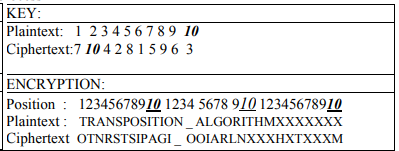
\includegraphics[width=0.9\textwidth]{imagenes/Transposition.png}
\caption{Transposition Cipher}
\label{table:1}
\end{table}